\begin{table}[t]
\caption{Test-period forecast quality. MAE (gCO$_2$/kWh) by horizon band; empirical coverage (\%) of
nominal 90\% intervals from split conformal and ACI; mean ACI interval width. Naive = seasonal-naive MAE.
$^\dagger$GB with archived horizon-resolved operator (NESO) forecasts; NESO-st = the API's stored forecast.}
\label{tab:forecast}
\centering\scriptsize\setlength{\tabcolsep}{2.4pt}
\resizebox{\columnwidth}{!}{%
\begin{tabular}{llrrrrrrr}
\toprule
 & & \multicolumn{3}{c}{MAE by horizon (h)} & & \multicolumn{2}{c}{Cov.\ @90\%} & \\
\cmidrule(lr){3-5}\cmidrule(lr){7-8}
Region & Model & 1--6 & 7--24 & 25--48 & Naive & Split & ACI & Width \\
\midrule
GB-op$^\dagger$ & NESO & 17.6 & 23.6 & 27.4 & 51.0 & 91 & 90 & 118 \\
GB-op$^\dagger$ & LGBM & 29.1 & 44.9 & 53.9 & 51.0 & 86 & 90 & 200 \\
GB-25 & LGBM & 27.7 & 42.6 & 53.3 & 46.1 & 79 & 90 & 171 \\
GB-25 & NESO-st & 8.6 & 8.6 & 8.6 & 46.1 & 92 & 90 & 39 \\
CISO & LGBM & 23.7 & 29.5 & 34.2 & 31.5 & 86 & 90 & 135 \\
ERCO & LGBM & 44.5 & 60.1 & 66.4 & 71.6 & 71 & 86 & 230 \\
PJM & LGBM & 11.6 & 14.8 & 16.8 & 17.8 & 90 & 89 & 61 \\
MISO & LGBM & 26.9 & 41.8 & 47.6 & 51.8 & 66 & 88 & 154 \\
\bottomrule
\end{tabular}}
\end{table}


\section{Do Uncertainty-Aware Policies Help?}\label{sec:uncertainty}

\textbf{Forecasts and intervals (Table~\ref{tab:forecast}).}
NESO's operator forecast has MAE \res{FQ}{GBop}{F2}{maeh1to6} (1--6\,h) to
\res{FQ}{GBop}{F2}{maeh25to48}\,gCO$_2$/kWh (25--48\,h), well below our weather-free LightGBM
(\res{FQ}{GBop}{F1}{maeh1to6} and \res{FQ}{GBop}{F1}{maeh25to48}). Split-conformal intervals
under-cover when the test season differs from calibration (MISO: \res{FQ}{MISO}{F1}{covsplita1}\% at
nominal 90\%). ACI restores coverage to \res{FQ}{MISO}{F1}{covacia1}\%.

\textbf{A savings--harm dial (Fig.~\ref{fig:dial}).}
P4 values every deferred option at its hourly conformal upper bound. It cuts the harm rate by
\res{V2X}{ALL-u0.7}{P4}{harmcutvsPthree}\% relative to P3 but gives up
\res{V2X}{ALL-u0.7}{P4}{savinglossvsPthree} points of saving. It keeps only
\res{V2U}{ALL-S12-utiltarget0.7}{P4}{capture} of CG's saving (its CG capture ratio), because summing hourly upper
bounds over a multi-hour job ignores the strong correlation of errors across horizons. Replacing
the bound with forecast\,+\,$\lambda\cdot$width gives a continuum (orange curve). The decision-level
rule P7 calibrates the quantity that matters, the overestimate of the greedy choice's saving, and
traces a better curve as $\alpha$ varies. Neither is a free lunch: at 70\% utilisation P7 cuts harm by
\res{V2X}{ALL-u0.7}{P7}{harmcutvsPthree}\% for \res{V2X}{ALL-u0.7}{P7}{savinglossvsPthree} points of
saving. These rules are points on a trade-off curve, not winners.

\textbf{What the guarantee does and does not cover.}
Conformal calibration gives \emph{marginal} coverage over the calibration distribution of
decisions. For P7 that means, over all decisions where running now was possible,
$\Pr[\text{defer} \wedge \text{realised saving}<0] \le \alpha$. The harm rate is a
\emph{conditional} quantity, $\Pr[\text{harm}\mid\text{defer}]$, and is not bounded: when deferral is
rare, a small marginal violation budget concentrates on the few deferred jobs. Measured with the
exact denominator, the marginal rate of harmful voluntary deferrals stays at or below $\alpha$ in
\res{V2G}{a0.1}{P7}{marginalbelow} of 6 regions at $\alpha{=}0.1$ (maximum
\res{V2G}{a0.1}{P7}{marginalmax}\%) and at every other $\alpha$ tested. The conditional voluntary harm
rate is not bounded by it: at $\alpha{=}0.1$ it exceeds $\alpha$ in
\res{V2G}{a0.1}{P7}{conditionalabove} of 6 regions, most in MISO and PJM, reaching
\res{V2G}{a0.1}{P7}{conditionalmax}\% (MISO:
\res{V2G}{a0.1-MISO}{P7}{conditional}\% conditional vs.\ \res{V2G}{a0.1-MISO}{P7}{marginal}\% marginal).
In MISO and PJM, grid variation within the slack window is small relative to forecast error
(MISO's LightGBM forecast also carries a bias of \res{FQ}{MISO}{F1}{bias}\,g/kWh). The predicted saving then sits inside the noise,
the rule defers rarely, and the deferrals it does make are close calls. Contention harm (forced
shifts) is outside the guarantee altogether, because calibration sees an empty cluster.

\textbf{Re-planning does not compound harm.}
Hourly re-planning adds \res{V2R}{ALL}{P3vsP2}{ddecisions} deferral decisions per job for point
greedy, yet \emph{lowers} its harm rate by \res{V2R}{ALL}{P3vsP2}{harmdroppp} points: harm rose in
only \res{V2R}{ALL}{P3vsP2}{harmupfrac}\% of region--utilisation settings, and the same holds for P8
and P9. Across all policy pairs, decisions per job correlate only weakly with harm (Spearman
$\rho{=}$\res{V2R}{ALL}{decisions}{rhoharmrate}, $n{=}$\res{V2R}{ALL}{decisions}{n}). The exception is
P7. Every re-decision is another test, so re-planning raises its voluntary harm by
\res{V2R}{ALL}{P7vsP7-noreplan}{dharmvolpp} points and costs
\res{V2R}{ALL}{P7vsP7-noreplan}{savinglosspp} points of saving; P7 should decide once.

\begin{figure}[t]
\centering
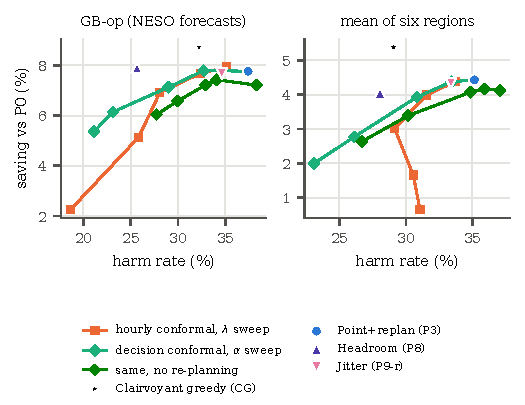
\includegraphics[width=\columnwidth]{figs/fig_dial.pdf}
\caption{Savings vs.\ harm at 70\% utilisation. Conformal rules sweep a trade-off curve ($\lambda$, $\alpha$);
the congestion-aware P8 lies above it.}
\label{fig:dial}
\end{figure}
